\documentclass{standalone}
\usepackage{tikz}
\usepackage{ctex,siunitx,ninecolors}
\setCJKmainfont{Noto Serif CJK SC}
\usepackage{tkz-euclide}
\usepackage{amsmath}
\usetikzlibrary{patterns, calc}
\usetikzlibrary {decorations.pathmorphing, decorations.pathreplacing, decorations.shapes,}
\begin{document}
\small
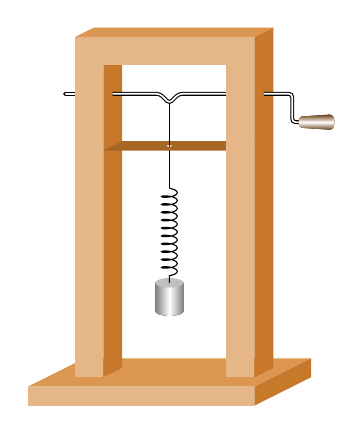
\begin{tikzpicture}[>=stealth, scale=1.2]
  % \useasboundingbox(-0.5,1.34)rectangle(7.55,-1.47);
  \fill[brown7](-1.5,-3.1)--++(2.4,0)--++(0.6,0.3)--++(-2.4,0)--cycle;
  \fill[brown8](-1.5,-3.1)rectangle++(2.4,-0.2);
  \fill[brown6](0.9,-3.3)--++(0.6,0.3)--++(0,0.2)--++(-0.6,-0.3)--cycle;
  \fill[brown6](-0.7,0.6)--++(0.2,0.1)--++(0,-3.6)--++(-0.2,-0.1)--cycle;
  \fill[brown7](-1.0,0.6)--(0.9,0.6)--++(0.2,0.1)--++(-1.9,0)--cycle;
  \draw(0,-0.55)--(0,-1);
  \fill[brown5,even odd rule](-0.7,-0.6)--++(0.2,0.1)--++(1.4,0)--++(-0.2,-0.1)--cycle (0,-0.55)ellipse(0.03 and 0.01);
  \draw(0,-0.1)--(0,-0.55);
  \draw[double,rounded corners=1.2pt](-0.6,0)--(-0.1,0)--(0,-0.1)--(0.1,0)--(0.6,0);
  \fill[left color=gray, right color=gray, middle color=white](0,-2.3)ellipse(0.15 and 0.05);
  \fill[left color=gray, right color=gray, middle color=white](-0.15,-2.0)rectangle(0.15,-2.3);
  \fill[lightgray](0,-2.0)ellipse(0.15 and 0.05);
  \draw[decorate,decoration={coil,aspect=0.3,segment length=1mm,amplitude=1mm}](0,-1.0)--(0,-2.0);
  \draw[double,rounded corners=1.2pt](-0.9,0)--++(-0.2,0);
  \draw(-1.1,0.0175)arc(90:270:0.0175);
  \fill[brown6](0.9,0.6)--++(0.2,0.1)--++(0,-3.6)--++(-0.2,-0.1)--cycle;
  \fill[brown8](-0.7,-3.0)rectangle(-1.0,0.6);
  \fill[brown8](0.6,-3.0)rectangle(0.9,0.6);
  \fill[brown8](-0.7,0.3)rectangle(0.6,0.6);
  \draw[double,rounded corners=1.2pt](1.0,0)--++(0.3,0)--++(0,-0.3)--++(0.1,0);
  \fill[top color=brown3,bottom color=brown3,middle color=white](1.4,-0.24)to[bend right=90](1.4,-0.36)--(1.7,-0.38)to[bend right=90](1.7,-0.22)--cycle;
\end{tikzpicture}
\end{document}
